%% 
%% Copyright 2007, 2008, 2009 Elsevier Ltd
%% 
%% This file is part of the 'Elsarticle Bundle'.
%% ---------------------------------------------
%% 
%% It may be distributed under the conditions of the LaTeX Project Public
%% License, either version 1.2 of this license or (at your option) any
%% later version.  The latest version of this license is in
%%    http://www.latex-project.org/lppl.txt
%% and version 1.2 or later is part of all distributions of LaTeX
%% version 1999/12/01 or later.
%% 
%% The list of all files belonging to the 'Elsarticle Bundle' is
%% given in the file `manifest.txt'.
%% 

%% Template article for Elsevier's document class `elsarticle'
%% with numbered style bibliographic references
%% SP 2008/03/01

\documentclass[preprint,12pt, a4paper]{elsarticle}

%% Use the option review to obtain double line spacing
%% \documentclass[authoryear,preprint,review,12pt]{elsarticle}

%% For including figures, graphicx.sty has been loaded in
%% elsarticle.cls. If you prefer to use the old commands
%% please give \usepackage{epsfig}

%% The amssymb package provides various useful mathematical symbols
\usepackage{amssymb}
%% The amsthm package provides extended theorem environments
%% \usepackage{amsthm}

%% The lineno packages adds line numbers. Start line numbering with
%% \begin{linenumbers}, end it with \end{linenumbers}. Or switch it on
%% for the whole article with \linenumbers.
\usepackage{lineno}
\usepackage{hyperref}




\journal{SoftwareX}

\begin{document}

\begin{frontmatter}

%% Title, authors and addresses

%% use the tnoteref command within \title for footnotes;
%% use the tnotetext command for theassociated footnote;
%% use the fnref command within \author or \address for footnotes;
%% use the fntext command for theassociated footnote;
%% use the corref command within \author for corresponding author footnotes;
%% use the cortext command for theassociated footnote;
%% use the ead command for the email address,
%% and the form \ead[url] for the home page:
%% \title{Title\tnoteref{label1}}
%% \tnotetext[label1]{}
%% \author{Name\corref{cor1}\fnref{label2}}
%% \ead{email address}
%% \ead[url]{home page}
%% \fntext[label2]{}
%% \cortext[cor1]{}
%% \address{Address\fnref{label3}}
%% \fntext[label3]{}

\title{FAIMS Mobile: Flexible, open-source software for field research}

%% use optional labels to link authors explicitly to addresses:
%% \author[label1,label2]{}
%% \address[label1]{}
%% \address[label2]{}

\author[ahis]{Brian Ballsun-Stanton}
\ead{brian.ballsun-stanton@mq.edu.au}
\ead[url]{http://www.faims.edu.au}


\author[mhis]{Shawn A. Ross\corref{cor1}}
\ead{shawn.ross@mq.edu.au}

\author[ahis]{Adela Sobotkova}
\ead{adela.sobotkova@mq.edu.au}

\author[latrobe]{Penny Crook}
\ead{p.crook@latrobe.edu.au}

\address[ahis]{Department of Ancient History, Macquarie University, Sydney, Australia}
\address[mhis]{Big History Institute, Department of Modern History, Politics, and International Relations, and Department of Ancient History, Macquarie University, Sydney, Australia}
\address[latrobe]{Department of Archaeology, La Trobe University, Melbourne, Australia}



\cortext[cor1]{Corresponding author. Department of Ancient History, Macquarie University 2109 NSW, Australia. Tel.: +61 9850 7085.}


%% Corresponding author. Department of Ancient History, Macquarie University 2109 NSW, Australia. Tel.: +61 9850 7085. Email: shawn.ross@mq.edu.au. Other email addresses: brian.ballsun-stanton@mq.edu.au (B. Ballsun-Stanton),  adela.sobotkova@mq.edu.au (A. Sobotkova), and p.crook@latrobe.edu.au (P. Crook)
\begin{abstract}
%% Text of abstract 
FAIMS Mobile is a native Android application supported by an Ubuntu server facilitating human-mediated field research across disciplines. It consists of `core' Java and Ruby software providing a platform for data capture, which can be deeply customised using `definition packets' consisting of XML documents (data schema and UI) and Beanshell scripts (automation). Definition packets can also be generated using an XML-based domain specific language, making customisation easier. FAIMS Mobile includes features allowing rich and efficient data capture tailored to the needs of fieldwork. It also promotes synthetic research and improves transparency and reproducibility through the production of comprehensive datasets that can be mapped to vocabularies or ontologies as they are created.	

\end{abstract}

\begin{keyword}
%% keywords here, in the form: keyword \sep keyword
Android \sep Mobile software \sep Field research \sep Field science
%% PACS codes here, in the form: \PACS code \sep code

%% MSC codes here, in the form: \MSC code \sep code
%% or \MSC[2008] code \sep code (2000 is the default)

\end{keyword}

\end{frontmatter}

\linenumbers

%% main text



\section{Motivation and significance}

Many disciplines in the social sciences, humanities, and biological, earth, and environmental sciences depend upon data collected through human-mediated fieldwork. Such data might arise from excavation in archaeology, wildlife observation in ecology, soil sampling in environmental geochemistry, or subject interviews in oral history. Field research disciplines, however, often lack transparency and reproducibility, compromising the integrity of research results \cite{McNutt2016-dg}. Field data is often collected using an ad-hoc mix of hard copy, data fragments in various formats, and bespoke databases \cite{Borgman2015-zg, Kansa2010-qx, Kintigh2006-uf, Snow2006-nu}. Datasets, furthermore, are often trapped in hard-copy archives, local storage, or digital `silos', making them difficult to discover and limiting reinterpretation and reuse \cite{Blanke2010-ou}. Digital datasets are often highly variable, of poor quality, and incompatible. Deficiencies like these inhibit reuse of primary data and the aggregation of datasets from multiple studies for large-scale research \cite{Kintigh2006-uf, Kintigh2014-ks, McNutt2016-dg}. 

Insufficient attention has been paid to the development of software specifically designed for digital data collection during field research. Some tools exist for discrete tasks, such as measuring strikes and dips for structural geology (e.g., GeoCline or Rocklogger for Android), but more complex field data collection has been neglected. Most digital data collection in archaeology, for example, is accomplished either using a combination of generic and repurposed mobile and desktop applications (e.g., multimedia, office productivity, GIS, database, or social survey software), or by building bespoke applications. Both approaches have severe limitations \cite{Sobotkova2016-mx}. Bespoke software is expensive to build and maintain, placing it beyond the reach of all but the best-funded projects and organisations (e.g., iDig, created by the American School of Classical Studies at Athens: \url{http://idig.tips/} (Archived at: \url{https://perma.cc/23PS-6567}); \cite{Fee2016-nn}). Repurposed software requires field researchers to make do with applications, designed for other contexts, which lack critical features but still require extensive customisation (cf. the use of a suite of iOS applications at Pompeii \cite{Ellis2016-vh}, or Ben Carter's combination of KoBoToolbox, PostGIS, QGIS, LibreOffice Base, and pgadminIII \cite{Carter2016-jm}). 

FAIMS Mobile, conversely, is `generalised' software which combines features required for field research with sufficient customisability to allow its use across disciplines, appealing to a large enough user base to support its development and have a meaningful impact on research (see Section 4 below; cf. \cite{Sobotkova2016-mx}). It is designed for offline use, unlike most other generalised field data collection software such as ARK, Heurist, or Kora \cite{Gordon2016-xf}, which all require a continuous connection to a server. FAIMS Mobile is open-source software developed by the Field Acquired Information Management Systems Project, an e-research infrastructure project based at Macquarie University, Sydney, Australia. It is mature software that has been under development since 2012 (see: \cite{Ross2015-mo, Ross2013-dz, Sobotkova2015-lq}). 

FAIMS Mobile is most comparable to Open Data Kit (ODK) (\url{https://opendatakit.org/}, \url{https://perma.cc/9BGB-8RUT}) and its variants, but is differentiated by its lineage. ODK was designed for social surveys, where an investigator asks questions of a interviewee. FAIMS originated in archaeology, where an investigator records observations about: things in the material world, relationships between those observations, and metadata contextualising the collection of those observations. Both projects are open-source, Java-based data collection platforms customised using XML-based domain specific languages. ODK also offers simpler but more restrictive customisation using ODK Build (an HTML5 drag-and-drop interface), XLSForm (a tool that uses an Excel file to build a form), or third-party, GUI-based applications like KoBoToolbox. FAIMS, conversely, supports more profound customisation without modification of core software. It also includes features not found in ODK: more nuanced relationships between entities, bi-directional synchronisation across all devices (a feature in ODK 2.0 Tool Suite, which is in alpha release), use of an append-only datastore that provides a version history for all records, support for a wider range of external sensors and peripherals like label printers (`ODK Sensors' is in alpha release), a more sophisticated data export framework, and more advanced geospatial data operations (compared to GeoODK and its derivatives). FAIMS also has richer and more granular help and metadata capture. In short, FAIMS is more customisable and has more fieldwork-specific features than ODK, but as a result customisation is more entailed. Field research projects, especially in liminal disciplines such as linguistics or oral history, would be wise to evaluate both platforms.


\subsection{Experimental setting}


FAIMS Mobile is designed to collect heterogenous data of various types (structured, free text, geospatial, multimedia), and accompanying metadata, produced using arbitrary methodologies during human-mediated field research. It requires customisation to instantiate a project-specific data model, user interface, and workflow, but it addresses problems shared across field-based projects, such as provision of a mobile GIS and automated synchronisation across multiple devices in a network-degraded environment. The FAIMS Project provides customisation services under a typical open-source revenue model \cite{Kelly2008-sb}. We also provide `User to Developer' documentation (\url{https://github.com/FAIMS/UserToDev}, archived at: \url{https://perma.cc/M4B3-JJEA}) to support do-it-yourself customisation.

During a typical FAIMS-led deployment, researchers work with FAIMS Project staff to articulate their data model and workflow. A developer then renders that methodology into a `definition packet' of files that produce a `module' (i.e., an implementation of FAIMS Mobile customised for a particular project). Separate definition packet files offer nuanced control the data schema (XML), the user interface (XML and CSS), and automation and logic (Beanshell). The interface can also be translated into multiple languages using a (plain text) localisation file. Completed modules are deployed to a local or online Ubuntu server, and from there onto as many Android devices as needed (after the core mobile application is installed, e.g. from Google Play). Data is then collected using those devices, which can operate fully offline, and synchronised opportunistically when a connection to the server is available. Data can be validated at the time of entry on the device, or later on the server. At the end of data collection, data is exported in the user's desired format by means of a customisable exporter. Three deployment case studies have been published in Sobotkova, et al., 2016\cite{Sobotkova2016-mx}.

Alternatively, FAIMS has developed a XML-based domain specific language (DSL) to simplify customisation. Using this DSL, a single file is used to generate a complete definition packet, at the expense of some loss of independent control over each element of a customisation (data schema, UI, automation). 

In addition to deployments conducted by the FAIMS team, projects have independently customised FAIMS Mobile themselves using both the detailed approach of producing an entire definition packet and the simplified DSL-based method\cite{Good2016-gf, Kiley2016-sf}. Users who are satisfied with one of the many modules in our GitHub library (\url{https://github.com/FAIMS}) can also simply instantiate an existing customisation.

\section{Software description}


FAIMS Mobile is open-source, customisable software designed specifically to support field research across many domains. It allows offline collection of structured, text, multimedia, and geospatial data on multiple Android devices, and is built around an append-only datastore that provides complete version histories. It includes customisable export to existing databases or in standard formats, supported by features that facilitate data compatibility. Finally, it is designed for rapid prototyping using and easy redeployability to reduce the costs of implementation. 


\subsection{Software Architecture}



FAIMS Mobile consists of `core' software written in Java and Ruby, customised to particular field deployments using reusable definition packets consisting of XML, Beanshell, and CSS files (which can be generated from a single file written in an XML-based DSL). More specifically, FAIMS uses the following technologies:

\begin{itemize}
\item Javarosa to render native Android UI elements at runtime;
\item Sqlite3 to store an attribute-key-value datastore (with data schemas definable at runtime);
\item An append-only data model inspired by Google's Protobufs;
\item Beanshell to provide runtime scripting via calls to an underlying Java API;
\item Spatialite to encode geospatial data in the datastore;
\item Nutiteq to render geospatial data;
\item NativeCSS to style android-native elements;
\item Antlr3 as a grammar parser for identifiers; and a
\item A Ruby on Rails / Apache stack to provide a server for synchronisation, version review, user management, and similar tasks, which can be hosted online or on modest hardware in the field.
\end{itemize}

We developed this architecture to meet two fundamental requirements: (1) the software had to accommodate a wide range of research designs, data schemas, and workflows, and (2) the software had to accommodate extremely variable structured, free text, multimedia, and geospatial data. We needed to build a system capable of rendering and recording arbitrary field data, since individual `data loggers' tied to a particular methodologies (even if extensible) and built as separate mobile applications would not appeal to a large enough audience to warrant the investment required. 

Our Android client can render definition packets at runtime to instantiate an arbitrary data collection methodology (schema and workflow), save records to a datastore, and opportunistically synchronize that data with a server and from there to other mobile devices. This distinction between the `core' client and the definition packet resembles the one between a web browser and a website. A browser contains many sophisticated engines for rendering the page, its interactivity, and its styling, but does not have content. A website uses the HTML engine provided by the browser to display its specific content. 

Four years of deployment experience revealed the importance of quality assurance, something too often neglected in academic software \cite{Might2010-fo, Sun2012-ub}. Each customisation and deployment is, indeed, a miniature software development project \cite{Sobotkova2016-mx}. Due to the need for significant QA per deployment, FAIMS Mobile 2.5+ supports Robotium for unit and integration tests on customised data collection modules, such that large amounts of test data can be automatically added via the normal user interface. This allows users to load-test their modules under simulated field conditions. 

\subsection{Software Functionalities}



FAIMS Mobile improves field research by providing a wide range of features that specifically address the needs of field research across disciplines, while facilitating the production of compatible datasets from  heterogeneous data structures and workflows. These features include:

\begin{itemize}
\item Deep customisation of data schema, user interface, and automation using either a packet of XML, Beanshell, and CSS documents for nuanced control, or a single file in an XML-based domain-specific language for ease of deployment. Definition document(s) are separate from core software, making modification and reuse easier.
\item Collection of various data types within a single record, including structured data, geospatial data, free text, sensor-produced multimedia, and file attachments.
\item Automated, bidirectional synchronisation of all data across an unlimited number of devices using a local or online server. Replication of the entire datastore on each device, not caching, provides robust offline capability. 
\item Opportunistic synchronisation whenever a connection is available, allowing devices to work in network-degraded environments or offline for extended periods of time. 
\item Configurable synchronisation of multimedia files; e.g., to reduce device storage demands, a full-resolution image can be kept on the server while only thumbnails are copied to devices.
\item Defaults, flow logic, hierarchical selections, dynamic UI (expand, collapse, hide, or show input fields), and other advanced data collection features.
\item Mobile GIS supporting raster and vector data, layer management, legacy data visualisation, and point, line, and polygon creation and editing. Multiple records can be linked to a single shape, or multiple shapes to a single record.
\item Offline mapping. Base maps and legacy data are uploaded to the server and pushed to all devices. Geospatial data (vectors) created in the field is synchronised across all devices. 
\item `Annotation' and `certainty' fields attached to every record. The former allows the collection of granular metadata (mimicking the `margins of the page' in paper recording), while the latter allows users to record their confidence in an observation. 
\item Internal and external sensor and peripheral support. All internal device sensors can be called (e.g., camera, microphone, GPS, etc.). External Bluetooth devices like GPS receivers, USB / HID devices like digital balances and calipers, and Bluetooth or USB label printers can be connected.
\item Multilingual support using a plain-text localisation file.
\item An append-only datastore providing a full revision history, including the ability to review and reverse changes to records selectively.
\item Mobile device and server-side validation.
\item Aids to good practice including contextual HTML help, `picture dictionaries' (selections based on images), and selection trees that can guide users through complex processes.
\item Embedding of URIs into controlled vocabularies or other elements to link them to shared vocabularies, thesauri, or ontologies.
\item Customisable export to desktop software, pre-existing databases, or online data services (using SQL queries).
\end{itemize}


\subsection{Sample code snippets analysis}


While a detailed discussion of module code is out of scope for this paper, two documents discuss module creation from start to finish. `FAIMS User to Developer Documentation' (\url{https://github.com/FAIMS/UserToDev}, archived at: \url{https://perma.cc/M4B3-JJEA}) is designed to walk users through the creation of a module from first principles. The `FAIMS Cookbook' is a tutorial covering data structures and API (\url{https://faimsproject.atlassian.net/wiki/x/RgAu}, archived: \url{https://perma.cc/H6XJ-X6E2}).

\section{Illustrative Examples}


\begin{figure}[!htb]
\minipage{0.49\textwidth}
	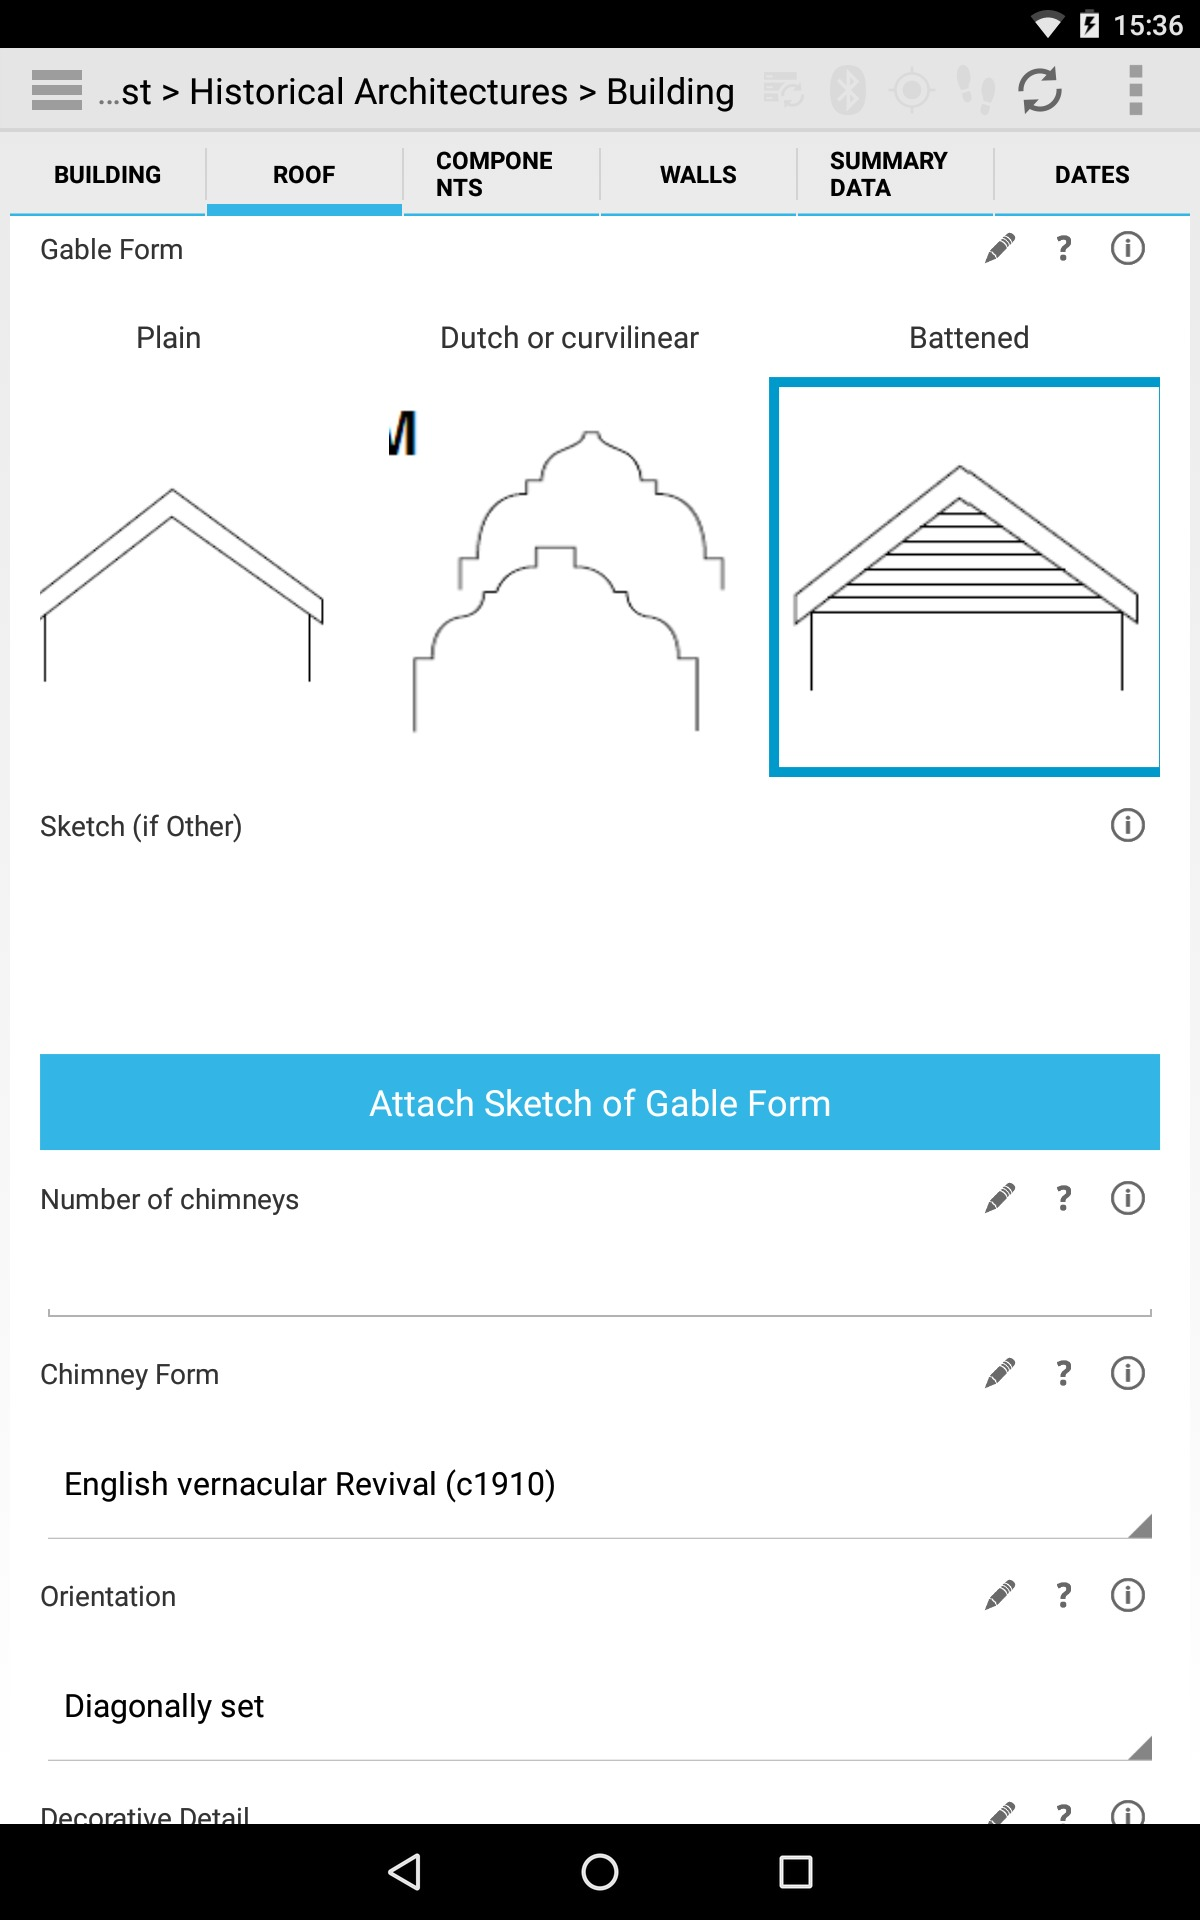
\includegraphics[width=\linewidth]{image-0.jpg}
	\caption{Structured data recording: including dropdowns, numeric fields, checkboxes, radio buttons, and `picture dictionaries'}
	\label{fig:img0}
\endminipage\hfill
\minipage{0.49\textwidth}
	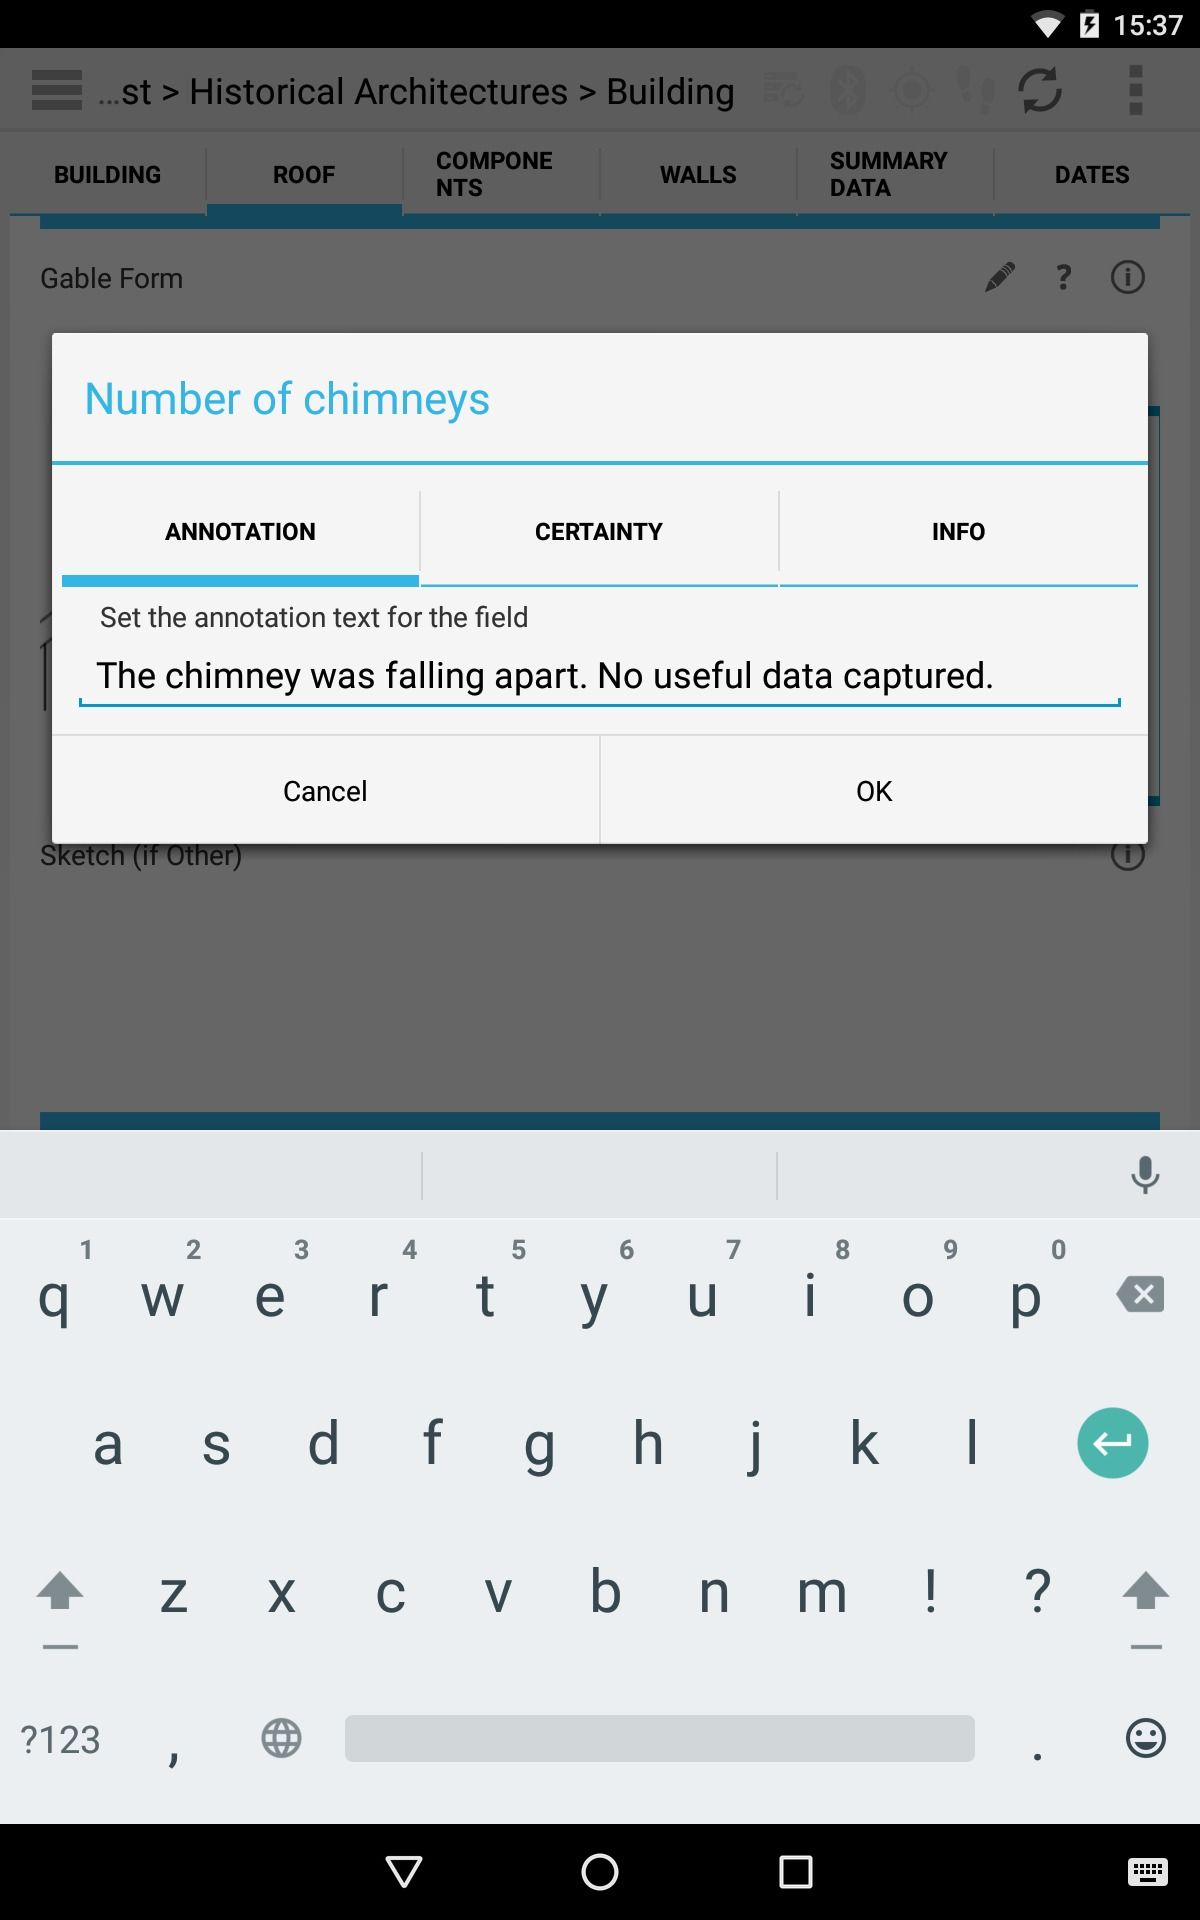
\includegraphics[width=\linewidth]{image-1.jpg}
	\caption{FAIMS has metadata such as annotations (digital `scribbling on the margin') and certainty. Granular, contextualised, HTML-format help (`info') is also delivered using this interface}
	\label{fig:img1}
\endminipage\hfill

\end{figure}

FAIMS offers a variety of ways to record data (Fig.~\ref{fig:img0}), all of which can be arranged hierarchically. All fields, regardless of datatype, allows for the recording of relevant metadata (Fig.~\ref{fig:img1}).


\begin{figure}[!htb]
\minipage{0.49\textwidth}
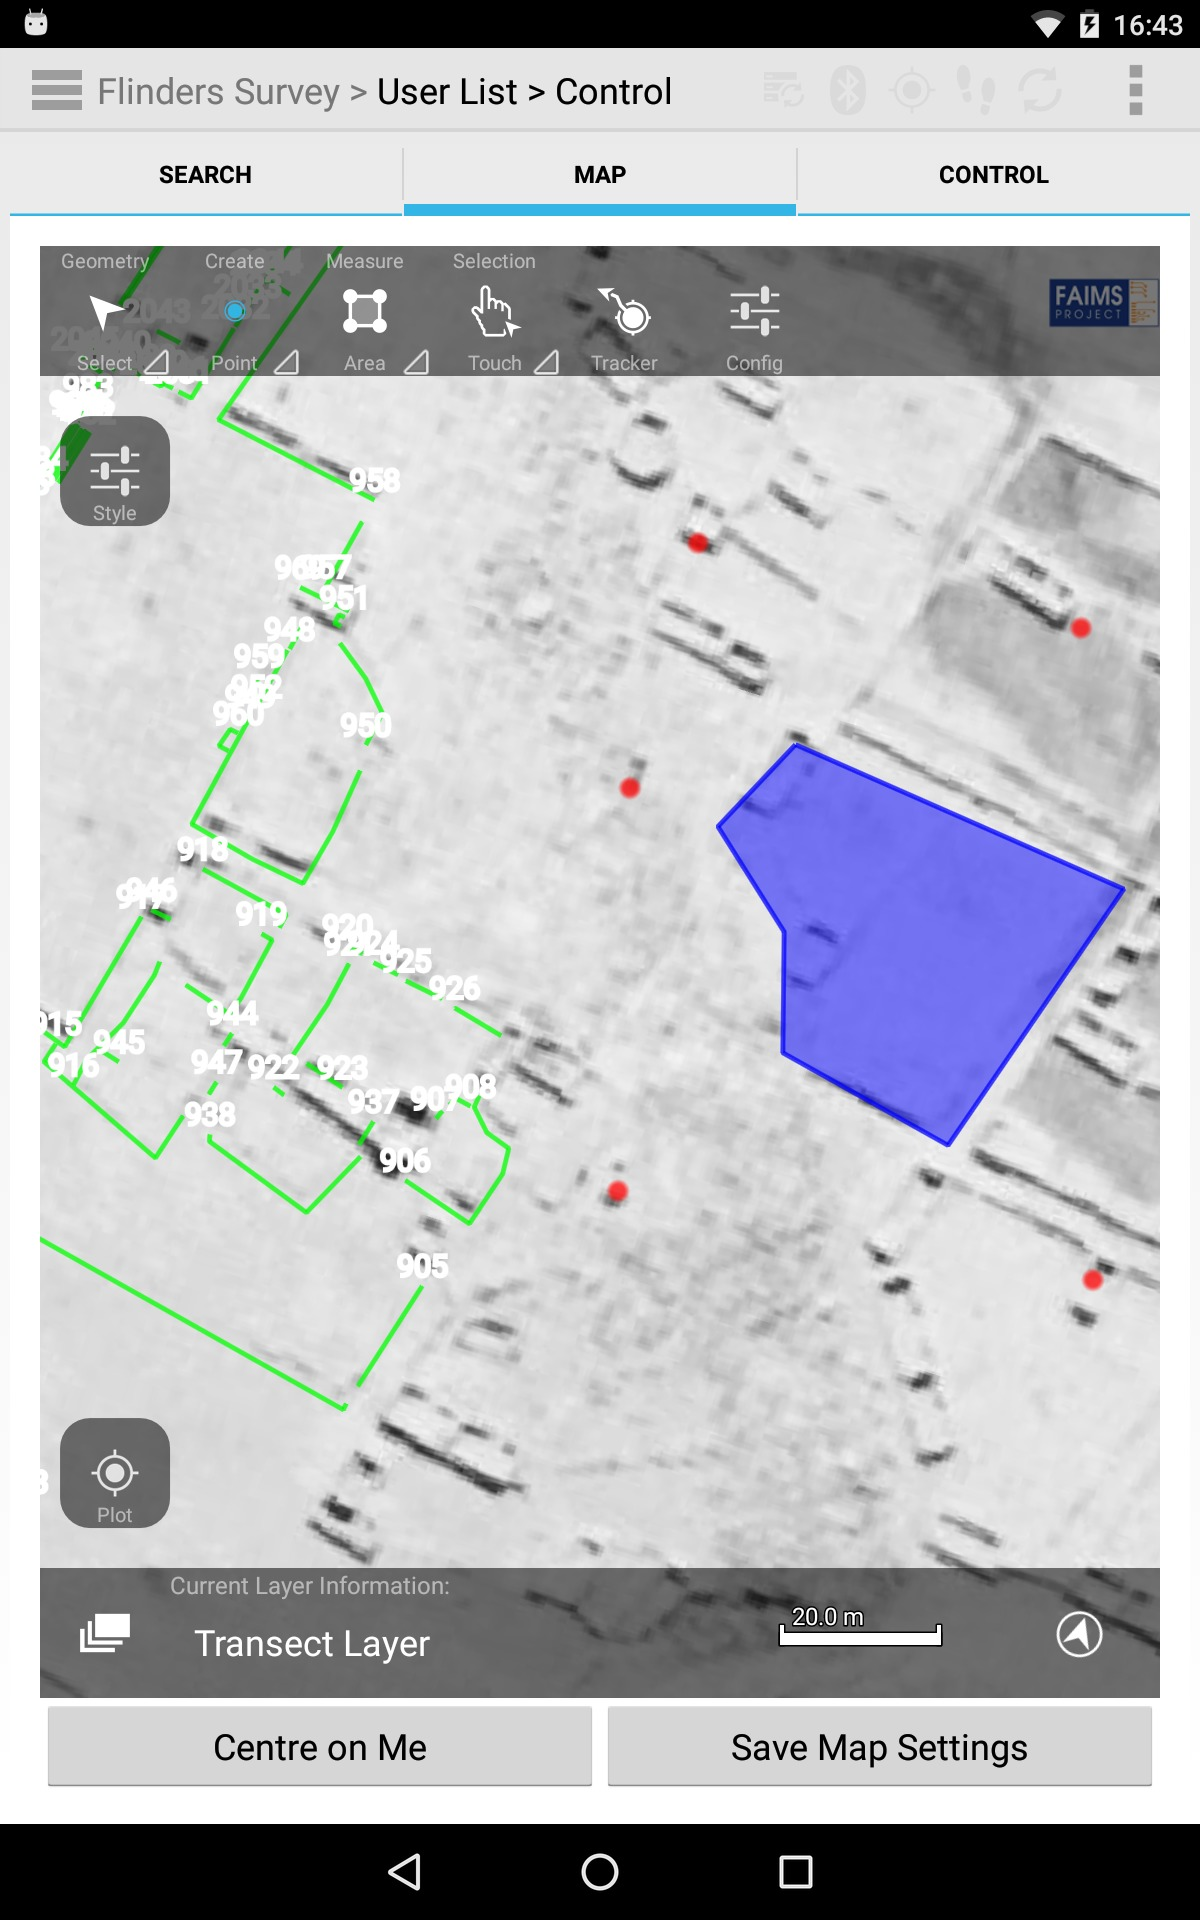
\includegraphics[width=\linewidth]{image-2.jpg}
	\caption{FAIMS Mobile can render layers of georeferenced raster files like satellite images}
	\label{fig:img2}
\endminipage\hfill
\minipage{0.49\textwidth}
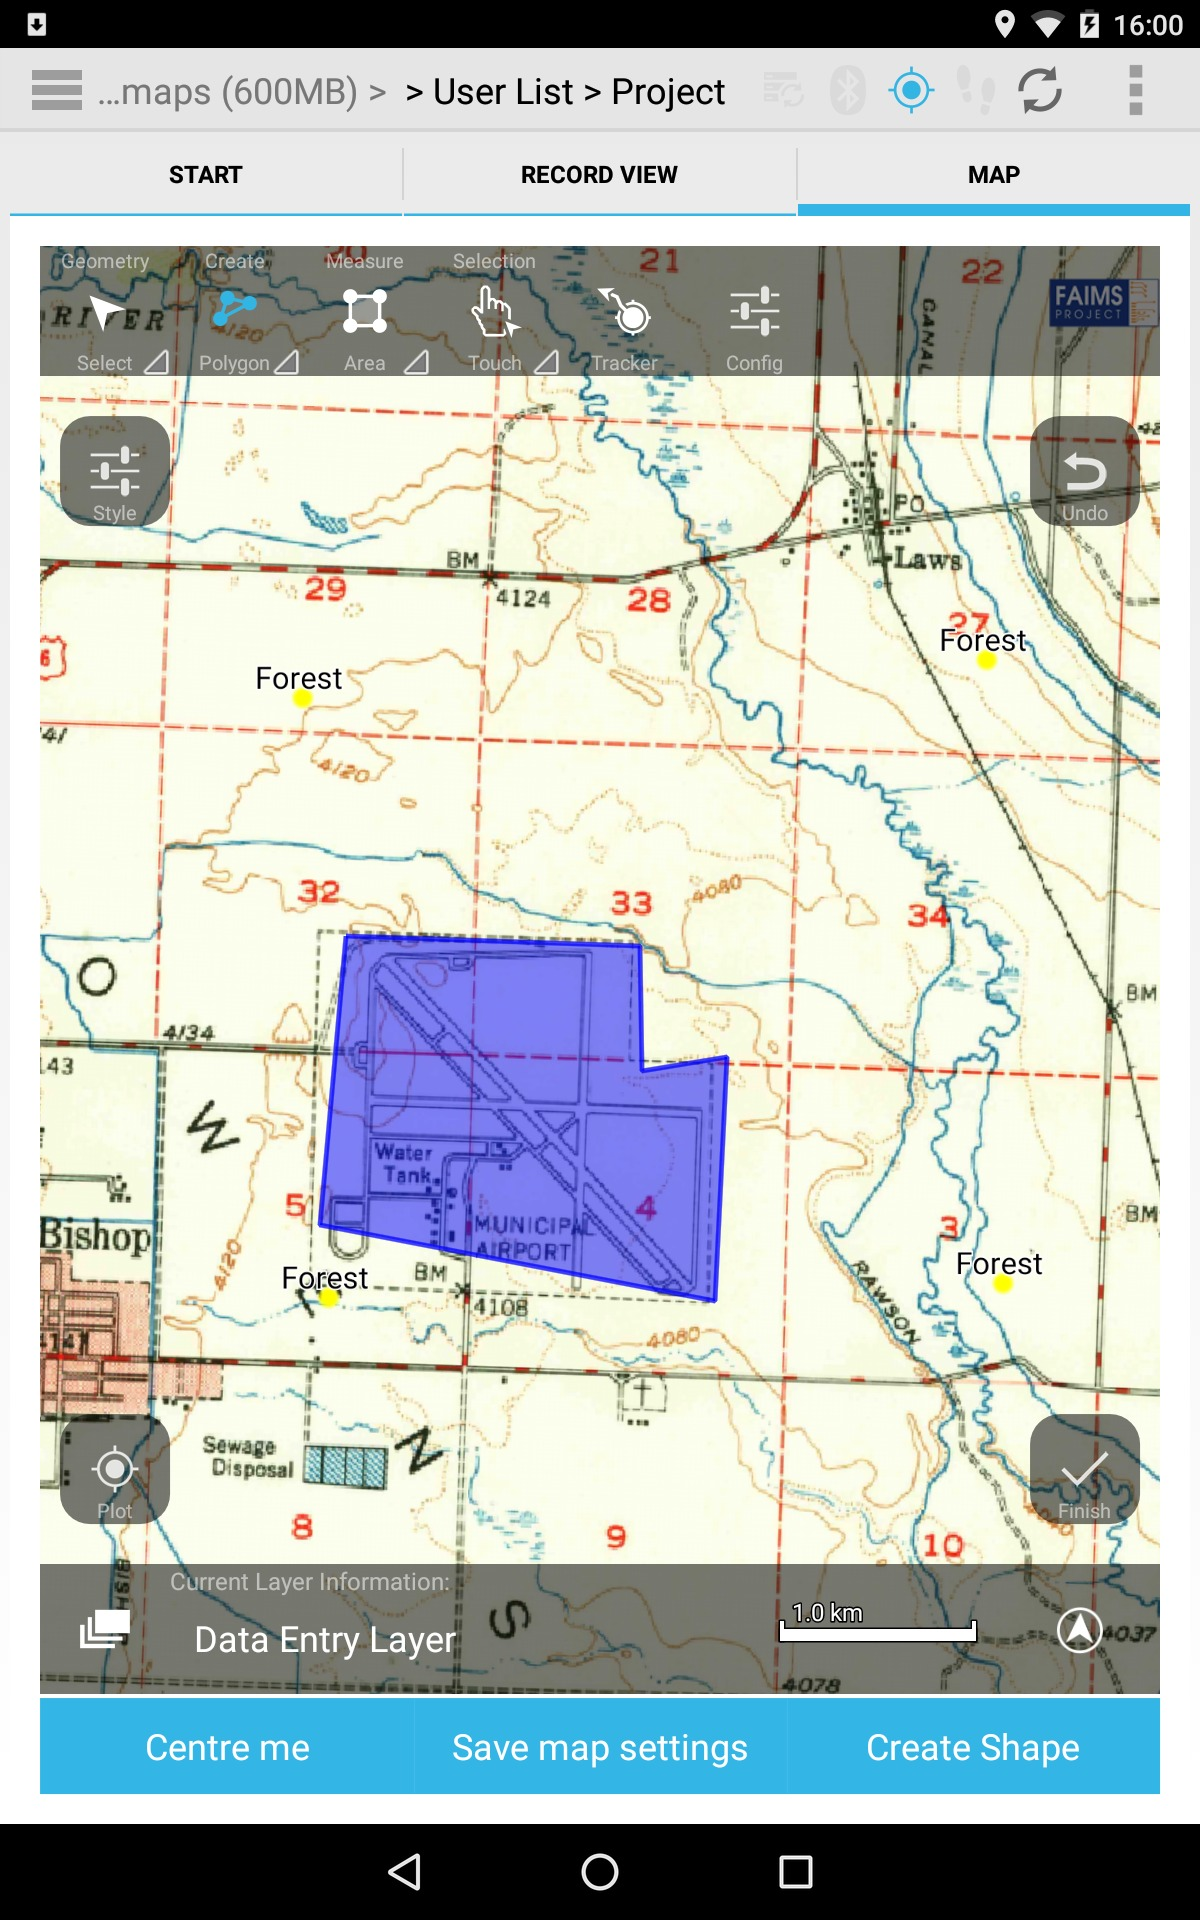
\includegraphics[width=\linewidth]{image-3.jpg}
	\caption{And topo maps}
	\label{fig:img3}
\endminipage\hfill

\end{figure}



Field research often requires spatial data capture and visualisation. FAIMS has GIS rendering capabilities for raster (Figs.~\ref{fig:img2},~\ref{fig:img3}), or vector data (blue polygons in both). Vector data can be created in the field and automatically bound to a record. 


\section{Impact}



FAIMS allows the efficient collection of field data, dramatically reducing or eliminating manual digitisation (see \cite{Sobotkova2016-mx}). Near-real-time availability of data from multiple devices for review also provides immediate error detection (especially when combined with validation). The software is free (as in speech), customisable, and extensible, accommodating arbitrary research designs. It is also purpose-built for field research. Such research represents only a fraction of the market for consumer or business software, and is unlikely to drive its development - whereas it is the sole focus of FAIMS. Finally, FAIMS Mobile is community driven; if current or potential users request new features, they can be implemented (within resource constraints). Researchers can also build and share their own customisations \cite{Sobotkova2016-mx}, while organisations with sufficient development capacity are welcome to contribute directly to the core software.

Beyond the immediate needs of users, FAIMS Mobile improves research practice and data management. URIs can be embedded in controlled vocabularies and other elements\cite{Sobotkova2015-lq}, connecting them to linked open data sources (e.g., species information can be linked to the Encyclopedia of Life\cite{Wilson2003-xx}). Localisation can be used to `translate' a local language of practice to a standard vocabulary (e.g., archaeological `context' or `locus' can be translated to `statigraphic unit' - and then linked to an online ontology). Customisable data export can format data for existing services or standards (e.g., archaeological records can be exported not only as shapefiles, CSVs, or a 3NF relational database for incorporation into an existing geodatabase, but also as XML or GeoJSON for ingest into domain-specific repositories like Open Context). Perhaps most importantly, comprehensive, rather than selective, datasets can be created and exported for publication, improving transparency and reproducibility. Together, these features that improve data compatibility across projects, facilitating large-scale field research. 

FAIMS Mobile makes digital recording a more feasible and less costly option for researchers \cite{Sobotkova2016-mx, Sobotkova2015-lq}. The core software does the `heavy lifting' of field recording (data storage, bi-directional synchronisation, GIS, etc.), and can be customised by leveraging either the control offered by the full definition packet or the efficiency of the DSL module generator. An experienced developer can rapidly prototype a recording system if data and workflow models are available (well-scoped systems of moderate complexity can be prototyped in one to two developer-days). Reuse and modification of existing customisations from a growing, openly-licensed online library (leveraging version control systems like GitHub) also helps to reduce deployment costs\cite{Ross2015-mo}. Customisation of FAIMS Mobile is therefore less expensive than production of bespoke mobile applications, and competitive with deploying the suite of generic tools field research requires: a DBMS, GIS, social survey software, multimedia management software, note-taking software, etc. \cite{Carter2016-jm}. At the same time, FAIMS offers better integration of different data types and requires fewer compromises on the part of the researcher compared to generic tools. Since FAIMS is also easier to redeploy than customised suites of generic tools, it allows practices and innovations to be readily shared\cite{Ross2015-mo}.  

FAIMS Mobile has changed users' daily practice. Three case studies involving archaeological deployments \cite{Sobotkova2016-mx} indicate that users benefit from the increased efficiency of fieldwork, in that the time saved by avoiding digitisation more than offsets the time required to implement FAIMS and more data collected during fieldwork of a given length. Born-digital data avoided problems with delayed digitisation, which often occurred long after field recording when the context of of the record had been forgotten, or the person who made the record was no longer available. Researchers reported more complete, consistent, and granular data. They noted that information could be exchanged more quickly between excavators and specialists, which in one case improved `post-excavation reconstruction of the site' and facilitated the evaluation of patterns for meaning in another. They also observed that the process of moving from paper to digital required comprehensive reviews of field practice, during which knowledge implicit in existing systems to become explicit and data was modelled more carefully. By participating in a `miniature software development project', researchers gained familiarity with the strengths, limits, and demands of software, especially the need for extensive testing. The greatest challenge posed by the transition from paper has been the reallocation of time from the end of a project (digitisation) to the beginning (data modelling, development, and testing), even if an overall time-savings is realised. 

Although the transition to digital recording during fieldwork represents a significant socio-technical change, FAIMS Mobile has seen good uptake. Since 2013, FAIMS Mobile has been customised at least 40 times (by our team or independently), with 29 confirmed field deployments, nine of which included multiple field seasons (\url{https://faimsproject.atlassian.net/wiki/x/jBH3B} \url{https://perma.cc/RW4K-7X2U}). Considering only FAIMS-led development, approximately 300 users have logged over 10,000 hours in the application. Most uptake to date has been at large, multi-year projects that are still early in their lifecycle, so all FAIMS-related publications to date have focused on the software itself or the transition from paper-based to digital workflows. Fourteen archaeology, ecology, and history projects are scheduled for 2017 with an estimated usage of another 10,000 hours. A 2016-2017 New South Wales Research Attraction and Acceleration Program award is funding links to government resources (e.g., automated data submission to the Aboriginal Heritage Information Management System of NSW), making FAIMS Mobile more attractive to commercial users. This award is also funding community heritage and citizen science deployments, where members of the public can download preconfigured versions of FAIMS Mobile from Google Play (as discrete APKs; See our current set at \url{https://play.google.com/store/apps/developer?id=FAIMS%20Project} \url{https://perma.cc/574T-QSVD} which includeds a Burial Mounds data collector and a ADS Gravestones data collector with screenshots of both) to monitor archaeological remains or wildlife.


\section{Conclusions}

When they collect data digitally, field researchers often re-purpose mass-market or general-purpose software that was not specifically designed to meet their needs. Doing so often requires several tools (some of which are individually complex) to accommodate the rich and varied data they must collect. FAIMS Mobile offers an alternative. It is purpose-built for field research with extensive community input, including five years of iterative co-development with field researchers first in archaeology, and more recently in geoscience, history, and ecology. FAIMS Mobile offers an unparalleled range of features to support fieldwork, including collection of structured, free-text, multimedia, and geospatial data, deep customisability, mobile GIS, use of internal and external sensors, offline capability with opportunistic synchronisation using either an online or local server, full record version histories, multilingual support, certainties and annotations attached to individual fields, and rich contextual help. It includes customisable export to existing databases or in standard formats, supported by features that facilitate data compatibility. It is designed for rapid prototyping and easy redeployability to reduce the costs of implementation, leveraging online software version control systems like GitHub. FAIMS Mobile is community-driven, customisable, extensible software that can support the socio-technical transition from paper to digital in field research disciplines and facilitate the production of comprehensive, compatible datasets to improve synthetic research, transparency, and reproducibility.  


%% The Appendices part is started with the command \appendix;
%% appendix sections are then done as normal sections
\appendix

%% \section{}
%% \label{}

\section*{Acknowledgements}


We would like to thank the many individuals and organisation who have contributed the FAIMS Project since 2012. For a complete list of project sponsors and participants, see \url{https://www.faims.edu.au/}.

Funding: This work was supported by the National eResearch Collaboration Tools and Resources programme (RT043; V005), the Australian Research Council (LE140100151), the New South Wales Government Research Attraction and Acceleration Program, Macquarie University, Flinders University, La Trobe University, Southern Cross University, the University of Queensland, the University of Sydney, UNSW Australia, the Commonwealth Scientific and Industrial Research Organisation ON Prime programme, and fees paid by our users for consultation, customisation, deployment, and support services.


%% References:
%% If you have bibdatabase file and want bibtex to generate the
%% bibitems, please use
%%
\section*{References}


\bibliographystyle{elsarticle-num} 
\bibliography{FAIMS}

%% else use the following coding to input the bibitems directly in the
%% TeX file.

%%\begin{thebibliography}{00}

%% \bibitem{label}
%% Text of bibliographic item

%%\bibitem{}

%%\end{thebibliography}

\section*{Required Metadata}



%% To the people typesetting this. Do we want to perma.cc all of these uris? 


\begin{table}[!h]
\begin{tabular}{|l|p{6.5cm}|p{6.5cm}|}
\hline
\textbf{Nr.} & \textbf{Code metadata description} & \textbf{Please fill in this column} \\
\hline
C1 & Current code version & 2.5 \\
\hline
C2 & Permanent link to code/repository used for this code version & \begin{description}\item [Core Application] \url{https://github.com/FAIMS/faims-android}
\item [Server] \url{https://github.com/FAIMS/faims-web}
\item [Definition Packets] \url{https://github.com/FAIMS}  
\end{description}
\\
\hline
C3 & Legal Code License   & GPLv3 \\
\hline
C4 & Code versioning system used & git \\
\hline
C5 & Software code languages, tools, and services used & Java, Ruby, XML, SQLite, Spatialite, Javarosa, Antlr, Puppet, Apache, Imagemagick, God, Beanshell, gson, guice, Nutiteq (non-free), NativeCSS, Protobuf, Robotium \\
\hline
C6 & Compilation requirements, operating environments \& dependencies & Android Studio, Ubuntu 16.04, Nutiteq license (for non-watermarked GIS)\\
\hline
C7 & If available Link to developer documentation/manual & \begin{description} \item [Module Cookbook] \url{https://faimsproject.atlassian.net/wiki/x/RgAu} 
\item [Module Beanshell API] \url{https://faimsproject.atlassian.net/wiki/display/FAIMS/Program+Logic+Support}
\item [Developer documentation home] \url{https://faimsproject.atlassian.net/wiki/spaces/FAIMS/overview}
\item [`User to Developer' documentation] (\url{https://github.com/FAIMS/UserToDev}, archived at: \url{https://perma.cc/M4B3-JJEA}
\end{description}
 \\
\hline
C8 & Support email for questions & \url{support@fedarch.org} \\
\hline
\end{tabular}
\caption{Code metadata (mandatory)}

\end{table}




\begin{table}[!h]
\begin{tabular}{|l|p{6.5cm}|p{6.5cm}|}
\hline
\textbf{Nr.} & \textbf{(Executable) software metadata description} & \textbf{Please fill in this column} \\
\hline
S1 & Current software version & 2.5.20 \\
\hline
S2 & Permanent link to executables of this version  & \begin{description} \item [FAIMS Mobile]\url{http://www.fedarch.org/apk/}
\item [Google Play] \url{https://play.google.com/store/apps/details?id=au.edu.faims.mq.fieldresearch2&hl=en}
\item [Server Installer (wget and pipe to bash)] \url{https://raw.githubusercontent.com/FAIMS/faims-web/master/installer/puppetInstall.sh} \end{description}\\

\hline
S3 & Legal Software License & GPLv3 \\
\hline
S4 & Computing platforms/Operating Systems & Android, Ubuntu \\
\hline
S5 & Installation requirements \& dependencies & Android 6+, Ubuntu 16.04 \\
\hline
S6 & If available, link to user manual - if formally published include a reference to the publication in the reference list & `Getting started' guide and user documentation:
\url{https://faimsproject.atlassian.net/wiki/display/FAIMS/Getting+started+with+FAIMS+-+an+overview} \\
\hline
S7 & Support email for questions & support@fedarch.org\\
\hline
\end{tabular}
\caption{Software metadata (optional)}

\end{table}

\end{document}
\endinput
%%
%% End of file `SoftwareX_article_template.tex'.
